\documentclass[
	%parspace, % Add vertical space between paragraphs
	%noindent, % No indentation of first lines in each paragraph
	%nohyp, % No hyphenation of words
	%twoside, % Double sided format
	%draft, % Quicker draft compilation without rendering images
	%final, % Set final to hide todos
]{elteikthesis}[2021/09/20]

\epstopdfsetup{outdir=./}

\usepackage{url}

% The minted package is also supported for source highlighting
% See minted-intregration.tex for example
%\usepackage[newfloat]{minted}

% Document's metadata
\title{Kódvisszafejtés mélyhálókkal} % title
\date{2022} % year of defense

% Author's metadata
\author{Csertán András}
\degree{programtervező informatikus BSc}

% Superivsor(s)' metadata
\supervisor{Dr. Várkonyi Teréz Anna} % internal supervisor's name
\affiliation{egyetemi adjunktus} % internal supervisor's affiliation
%\extsupervisor{Külső Kornél} % external supervisor's name
%\extaffiliation{informatikai igazgató} % external supervisor's affiliation

% University's metadata
\university{Eötvös Loránd Tudományegyetem} % university's name
\faculty{Informatikai Kar} % faculty's name
\department{Programozáselmélet és Szoftvertechnológiai\\ Tanszék} % department's name
\city{Budapest} % city
\logo{elte_cimer_szines} % logo

% Add bibliography file
\addbibresource{thesis.bib}

% The document
\begin{document}

% Set document language
\documentlang{hungarian}
%\documentlang{english}

% List of todos (not in the final document)
%\listoftodos[\todolabel]

% Title page (mandatory)
\maketitle
% Topic declaration page (mandatory) - can also be attached instead
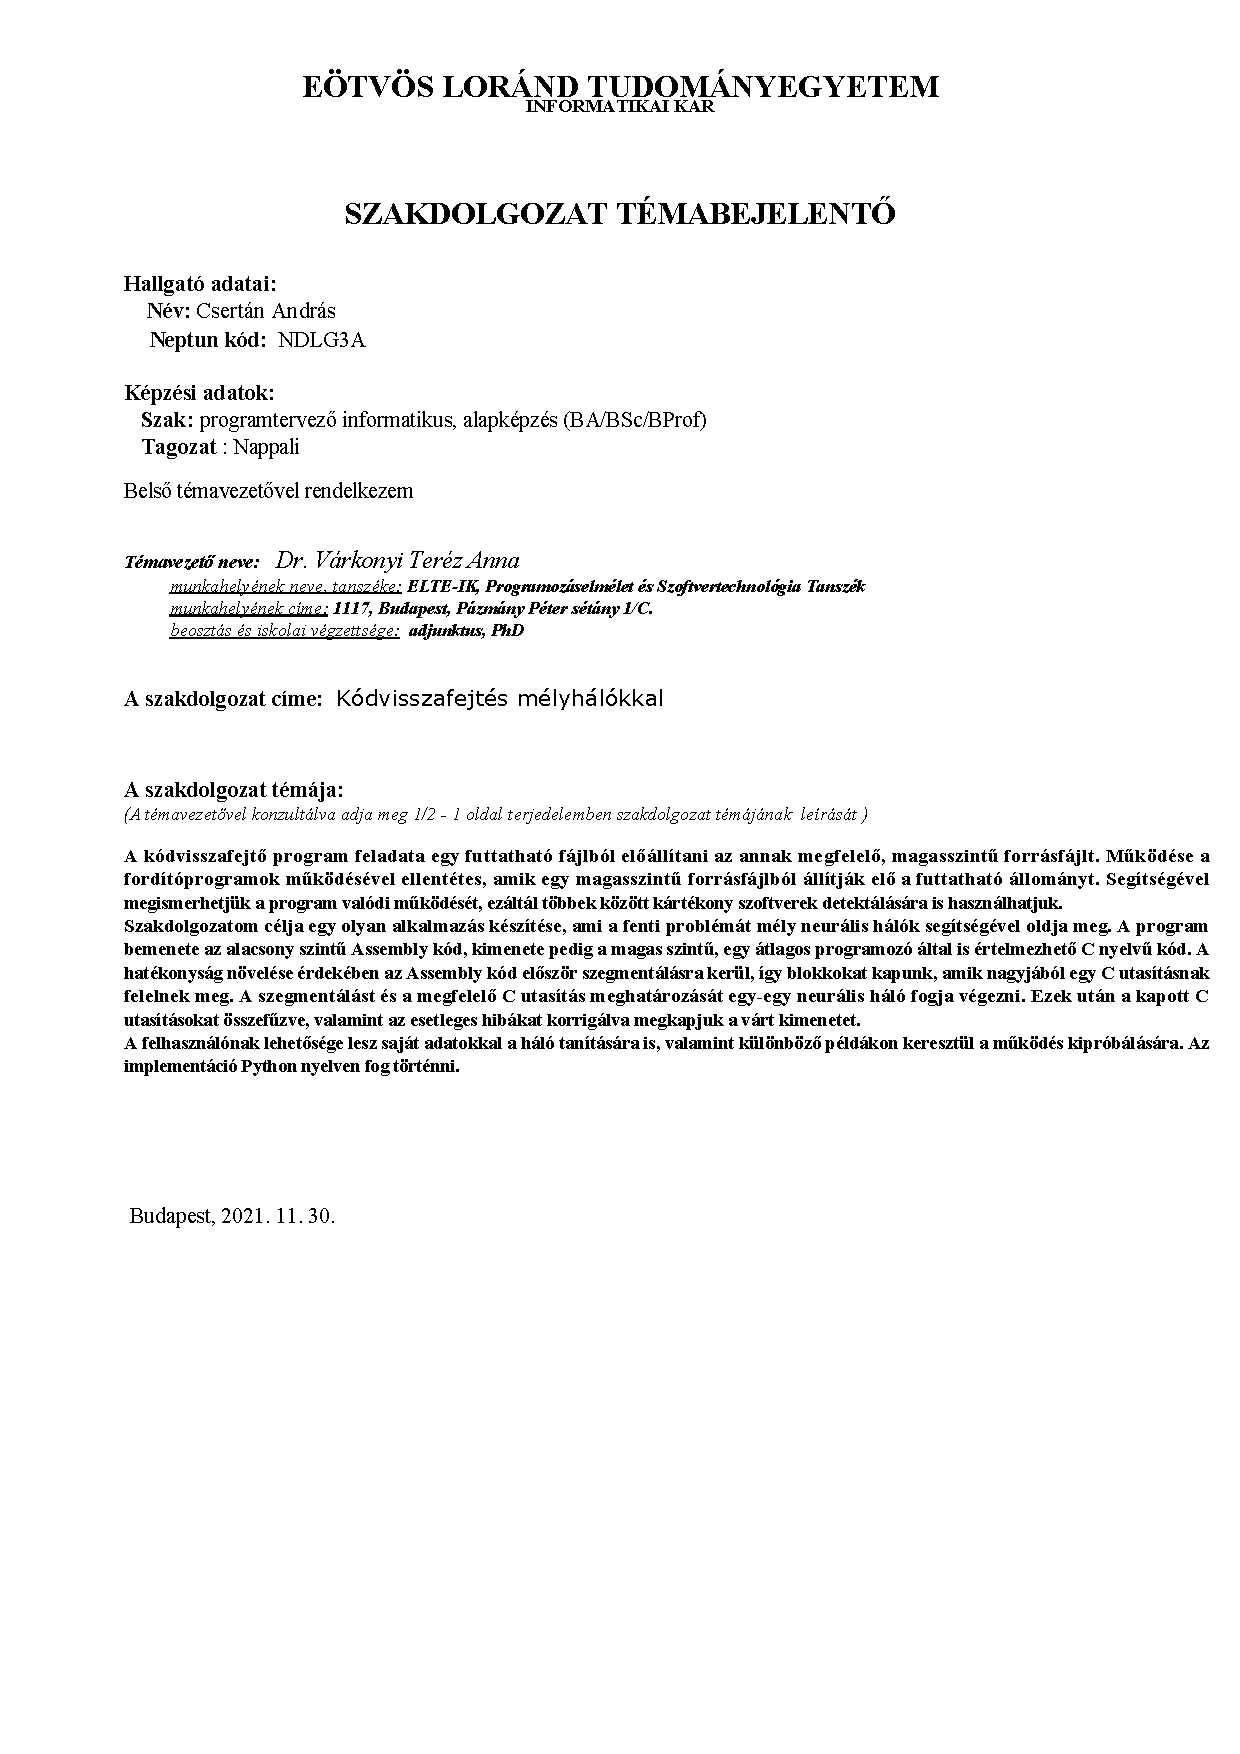
\includepdf{temabejelento.pdf}

% Table of contents (mandatory)
\tableofcontents
\cleardoublepage

% Main content
\chapter{Bevezetés}
\label{ch:intro}

A fordítóprogramok feladata a magas szintű programkód átalakítása a számítógép számára értelmezhető formára. Céljuk, hogy a programozó sokkal magasabb absztrakciós szinten fejezhesse ki szándékát, ezáltal megkönnyítve a szoftverfejlesztés folyamatát. A kódvisszafejtő programok működése ezzel ellentétes, az alacsony szintű, gépközeli kódot alakítják át magas szintű kóddá. Segítségével beleláthatunk a program forráskódjába akkor is, ha csak egy futtatható állomány áll rendelkezésre, ezáltal könnyebben megvédhetjük gépünket a kártékony szoftverektől.

A fenti feladat megoldására már léteznek különböző kódvisszafejtő prgoramok \cite{ghidra},\cite{binaryninja}, ugyanakkor ezek legnagyobb hátránya, hogy a fordítóprogramokhoz hasonlóan bonyolult szabályok alapján működnek. Ez azért probléma, mert ezen szabályokat minden programozási nyelv esetén külön meg kell fogalmazni, ami egy bonyolult és időigényes feladat.

Dolgozatomban egy olyan programot mutatok be, ami a fenti problémát a természetes nyelvfeldolgozásban használt gépi tanulási eszközökkel oldja meg. A neurális gépi fordítás az utóbbi években hatalmas fejlődésen ment keresztül[bert], így könnyen adódik, hogy ezen eredményeket fel lehetne használni a kódvisszafejtéshez, annyi különbséggel, hogy nem angolról németre, hanem például assembly-ről C-re fordítunk.\footnote{Majd látni fogjuk, hogy a programozási nyelvek sajátos szerkezete miatt sajnos nem alkalmazhatók egy az egyben a természetes nyelvek fordítása során elért eredmények.} Ezen módszer előnye, hogy nem szükséges hozzá programozók hosszú ideig munkája a különböző szabályrendszerek megalkotásához, valamint egy másik nyelvre való áttérés sem okoz különösebb nehézséget. Továbbá a különböző programkód generáló szoftvereknek\cite{??} hála, lényegében korlátlan mennyiségű adat áll rendelkezésre.

\cleardoublepage

\chapter{Felhasználói dokumentáció}
\label{ch:user}

Lorem ipsum dolor sit amet $\mathbb{N}$\nomenclature{$\mathbb{N}$}{Set of natural numbers}, consectetur adipiscing elit. Duis nibh leo, dapibus in elementum nec, aliquet id sem. Suspendisse potenti. Nullam sit amet consectetur nibh. Donec scelerisque varius turpis at tincidunt. Cras a diam in mauris viverra vehicula. Vivamus mi odio, fermentum vel arcu efficitur, lacinia viverra nibh. Aliquam aliquam ante mi, vel pretium arcu dapibus eu. Nulla finibus ante vel arcu tincidunt, ut consectetur ligula finibus. Mauris mollis lectus sed ipsum bibendum, ac ultrices erat dictum. Suspendisse faucibus euismod lacinia $\mathbb{Z}$\nomenclature{$\mathbb{Z}$}{Set of integer numbers}.


\section{Felsorolások}

Etiam vel odio ante. Etiam pulvinar nibh quis massa auctor congue. Pellentesque quis odio vitae sapien molestie vestibulum sit amet et quam. Pellentesque vel dui eget enim hendrerit finibus at sit amet libero. Quisque sollicitudin ultrices enim, nec porta magna imperdiet vitae. Cras condimentum nunc dui, eget molestie nunc accumsan vel.

\begin{itemize}
	\item Fusce in aliquet neque, in pretium sem.
	\item Donec tincidunt tellus id lectus pretium fringilla.
	\item Nunc faucibus, erat pretium tempus tempor, tortor mi fringilla neque, ac congue ex dui vitae mauris.
\end{itemize}

Donec dapibus sodales ante, at scelerisque nunc laoreet sit amet. Mauris porttitor tincidunt neque, vel ullamcorper neque pulvinar et. Integer eu lorem euismod, faucibus lectus sed, accumsan felis. Nunc ornare mi at augue vulputate, eu venenatis magna mollis. Nunc sed posuere dui, et varius nulla. Sed mollis nibh augue, eget scelerisque eros ornare nec.

\begin{enumerate}
	\item\label{step:first} Donec pretium et quam a cursus. Ut sollicitudin tempus urna et mollis.
	\item Aliquam et aliquam turpis, sed fermentum mauris. Nulla eget ex diam.
	\item Donec eget tellus pharetra, semper neque eget, rutrum diam \ref{step:first}.~lépés.
\end{enumerate}

Praesent porta, metus eget eleifend consequat, eros ligula eleifend ex, a pellentesque mi est vitae urna. Vivamus turpis nunc, iaculis non leo eget, mattis vulputate tellus. Maecenas rutrum eros sem, pharetra interdum nulla porttitor sit amet. In vitae viverra ante. Maecenas sit amet placerat orci, sed tincidunt velit. Vivamus mattis, enim vel suscipit elementum, quam odio venenatis elit\footnote{Phasellus faucibus varius purus, nec tristique enim porta vitae.}, et mollis nulla nunc a risus. Praesent purus magna, tristique sed lacus sit amet, convallis malesuada magna. 

\begin{description}
	\item[Vestibulum venenatis] malesuada enim, ac auctor erat vestibulum et. Phasellus id purus a leo suscipit accumsan.
	\item[Orci varius natoque] penatibus et magnis dis parturient montes, nascetur ridiculus mus. Nullam interdum rhoncus nisl, vel pharetra arcu euismod sagittis. Vestibulum ac turpis auctor, viverra turpis at, tempus tellus.
	\item[Morbi dignissim] erat ut rutrum aliquet. Nulla eu rutrum urna. Integer non urna at mauris scelerisque rutrum sed non turpis.
\end{description}

\subsection{Szoros térközű felsorolások}

Phasellus ultricies, sapien sit amet ultricies placerat, velit purus viverra ligula, id consequat ipsum odio imperdiet enim:
\begin{compactenum}
	\item Maecenas eget lobortis leo.
	\item Donec eget libero enim.
	\item In eu eros a eros lacinia maximus ullamcorper eget augue.
\end{compactenum}

\bigskip

In quis turpis metus. Proin maximus nibh et massa eleifend, a feugiat augue porta. Sed eget est purus. Duis in placerat leo. Donec pharetra eros nec enim convallis:
\begin{compactitem}
	\item Pellentesque odio lacus.
	\item Maximus ut nisl auctor.
	\item Sagittis vulputate lorem.
\end{compactitem}

\bigskip

Vestibulum ante ipsum primis in faucibus orci luctus et ultrices posuere cubilia Curae; Sed lorem libero, dignissim vitae gravida a, ornare vitae est.
\begin{compactdesc}
	\item[Cras maximus] massa commodo pellentesque viverra.
	\item[Morbi sit] amet ante risus. Aliquam nec sollicitudin mauris
	\item[Ut aliquam rhoncus sapien] luctus viverra arcu iaculis posuere
\end{compactdesc}


\section{Képek, ábrák}

Aliquam vehicula luctus mi a pretium. Nulla quam neque, maximus nec velit in, aliquam mollis tortor. Aliquam erat volutpat. Curabitur vitae laoreet turpis. Integer id diam ligula. Nulla sodales purus id mi consequat, eu venenatis odio pharetra. Cras a arcu quam. Suspendisse augue risus, pulvinar a turpis et, commodo aliquet turpis. Nulla aliquam scelerisque mi eget pharetra. Mauris sed posuere elit, ac lobortis metus. Proin lacinia sit amet diam sed auctor. Nam viverra orci id sapien sollicitudin, a aliquam lacus suscipit, \ref{fig:example-1}.~ábra:

\begin{figure}[H]
	\centering
	
\includegraphics[width=0.6\textwidth,height=100px]{elte_cimer_szines}
	\caption{Quisque ac tincidunt leo}
	\label{fig:example-1}
\end{figure}

\subsection{Képek szegélyezése}

Ut aliquet nec neque eget fermentum. Cras volutpat tellus sed placerat elementum. Quisque neque dui, consectetur nec finibus eget, blandit id purus. Nam eget ipsum non nunc placerat interdum.

\begin{figure}[H]
	\centering
	
\includegraphics[width=0.6\textwidth,height=100px,frame]{elte_cimer_szines}
	\caption{Quisque ac tincidunt leo}
\end{figure}

\subsection{Képek csoportosítása}

In non ipsum fermentum urna feugiat rutrum a at odio. Pellentesque habitant morbi tristique senectus et netus et malesuada fames ac turpis egestas. Nulla tincidunt mattis nisl id suscipit. Sed bibendum ac felis sed volutpat. Nam pharetra nisi nec facilisis faucibus. Aenean tristique nec libero non commodo. Nulla egestas laoreet tempus. Nunc eu aliquet nulla, quis vehicula dui. Proin ac risus sodales, gravida nisi vitae, efficitur neque, \ref{fig:example-2}.~ábra:

\begin{figure}[H]
	\centering
	\subcaptionbox{Vestibulum quis mattis urna}{
		
\includegraphics[width=0.45\linewidth]{elte_cimer_szines}}
	\hspace{5pt}
	\subcaptionbox{Donec hendrerit quis dui sit amet venenatis}{
		
\includegraphics[width=0.45\linewidth]{elte_cimer_szines}}
	\caption{Aenean porttitor mi volutpat massa gravida}
	\label{fig:example-2}
\end{figure}

Nam et nunc eget elit tincidunt sollicitudin. Quisque ligula ipsum, tempor vitae tortor ut, commodo rhoncus diam. Pellentesque habitant morbi tristique senectus et netus et malesuada fames ac turpis egestas. Phasellus vehicula quam dui, eu convallis metus porta ac.


\section{Táblázatok}

Nam magna ex, euismod nec interdum sed, sagittis nec leo. Nam blandit massa bibendum mattis tristique. Phasellus tortor ligula, sodales a consectetur vitae, placerat vitae dolor. Aenean consequat in quam ac mollis. 

\begin{table}[H]
	\centering
	\begin{tabular}{ | m{0.25\textwidth} | m{0.65\textwidth} | }
		\hline
		\textbf{Phasellus tortor} & \textbf{Aenean consequat} \\
		\hline \hline
		\emph{Sed malesuada} & Aliquam aliquam velit in convallis ultrices. \\
		\hline
		\emph{Purus sagittis} &  Quisque lobortis eros vitae urna lacinia euismod. \\
		\hline
		\emph{Pellentesque} & Curabitur ac lacus pellentesque, eleifend sem ut, placerat enim. Ut auctor tempor odio ut dapibus. \\
		\hline
	\end{tabular}
	\caption{Maecenas tincidunt non justo quis accumsan}
	\label{tab:example-1}
\end{table}

\subsection{Sorok és oszlopok egyesítése}

Mauris a dapibus lectus. Vestibulum commodo nibh ante, ut maximus magna eleifend vel. Integer vehicula elit non lacus lacinia, vitae porttitor dolor ultrices. Vivamus gravida faucibus efficitur. Ut non erat quis arcu vehicula lacinia. Nulla felis mauris, laoreet sed malesuada in, euismod et lacus. Aenean at finibus ipsum. Pellentesque dignissim elit sit amet lacus congue vulputate.

\begin{table}[htb]
	\centering
	\begin{tabular}{ | c | r | r | r | r | r | r | }
		\hline
		\multirow{2}{*}{\textbf{Quisque}} & \multicolumn{2}{ c | }{\textbf{Suspendisse}} & \multicolumn{2}{ c | }{\textbf{Aliquam}} & \multicolumn{2}{ c | }{\textbf{Vivamus}} \\
		\cline{2-7}
		& Proin & Nunc & Proin & Nunc & Proin & Nunc \\
		\hline \hline		
		Leo & 2,80 MB & 100\% & 232 KB & 8,09\% & 248 KB & 8,64\% \\
		\hline
		Vel & 9,60 MB & 100\% & 564 KB & 5,74\% & 292 KB & 2,97\% \\
		\hline
		Auge & 78,2 MB & 100\% & 52,3 MB & 66,88\% & 3,22 MB & 4,12\% \\
		\hline 
	\end{tabular}
	\caption[Rövid cím a táblázatjegyzékbe]{Vivamus ac arcu fringilla, fermentum neque sed, interdum erat. Mauris bibendum mauris vitae enim mollis, et eleifend turpis aliquet.}
	\label{tab:example-2}
\end{table}

\subsection{Több oldalra átnyúló táblázatok}

Nunc porta placerat leo, sit amet porttitor dui porta molestie. Aliquam at fermentum mi. Maecenas vitae lorem at leo tincidunt volutpat at nec tortor. Vivamus semper lacus eu diam laoreet congue. Vivamus in ipsum risus. Nulla ullamcorper finibus mauris non aliquet. Vivamus elementum rhoncus ex ut porttitor.

\begin{center}
	\begin{longtable}{ | p{0.3\textwidth} | p{0.7\textwidth} | }
		
		\hline
		\multicolumn{2}{|c|}{\textbf{Praesent aliquam mauris enim}}
		\\ \hline
		
		\emph{Suspendisse potenti} & \emph{Lorem ipsum dolor sit amet}
		\\ \hline \hline
		\endfirsthead % első oldal fejléce
		
		\hline
		\emph{Suspendisse potenti} & \emph{Lorem ipsum dolor sit amet}
		\\ \hline \hline
		\endhead % többi oldal fejléce
		
		\hline
		\endfoot % többi oldal lábléce
		
		\endlastfoot % utolsó oldal lábléce
		
		\emph{Praesent}
		& Nulla ultrices et libero sit amet fringilla. Nunc scelerisque ante tempus sapien placerat convallis.
		\\ \hline
		
		\emph{Luctus}
		& Integer hendrerit erat massa, non hendrerit risus convallis at. Curabitur ultrices, justo in imperdiet condimentum, neque tortor luctus enim, luctus posuere massa erat vitae nibh.
		\\ \hline
		
		\emph{Egestas}
		& Duis fermentum feugiat augue in blandit. Mauris a tempor felis. Pellentesque ultricies tristique dignissim. Pellentesque aliquam semper tristique. Nam nec egestas dolor. Vestibulum id elit quis enim fringilla tempor eu a mauris. Aliquam vitae lacus tellus. Phasellus mauris lectus, aliquam id leo eget, auctor dapibus magna. Fusce lacinia felis ac elit luctus luctus.
		\\ \hline
		
		\emph{Dignissim}
		& Praesent aliquam mauris enim, vestibulum posuere massa facilisis in. Suspendisse potenti. Nam quam purus, rutrum eu augue ut, varius vehicula tellus. Fusce dui diam, aliquet sit amet eros at, sollicitudin facilisis quam. Phasellus tempor metus vel augue gravida pretium. Proin aliquam aliquam blandit. Nulla id tempus mi. Fusce in aliquam tortor.
		\\ \hline
		
		\emph{Pellentesque}
		& Donec felis nibh, imperdiet a arcu non, vehicula gravida nibh. Quisque interdum sapien eu massa commodo, ac elementum felis faucibus.
		\\ \hline
		
		\emph{Molestie}
		& Cras ullamcorper tellus et auctor ultricies. Maecenas tincidunt euismod lectus nec venenatis. Suspendisse potenti. Pellentesque pretium nunc ut euismod cursus. Nam venenatis condimentum quam. Curabitur suscipit efficitur aliquet. Interdum et malesuada fames ac ante ipsum primis in faucibus.
		\\ \hline
		
		\emph{Vivamus semper}
		& In purus purus, faucibus eu libero vulputate, tristique sodales nunc. Nulla ut gravida dolor. Fusce vel pellentesque mi, vel efficitur eros. Nunc vitae elit tellus. Sed vestibulum auctor consequat. 
		\\ \hline
		
		\emph{Condimentum}
		& Nulla scelerisque, leo et facilisis pretium, risus enim cursus turpis, eu suscipit ipsum ipsum in mauris. Praesent eget pulvinar ipsum, suscipit interdum nunc. Nam varius massa ut justo ullamcorper sollicitudin. Vivamus facilisis suscipit neque, eu fermentum risus. Ut at mi mauris.
		\\ \hline
		
		\caption{Praesent ullamcorper consequat tellus ut eleifend}
		\label{tab:example-3}		
	\end{longtable}
\end{center}
\cleardoublepage

\chapter{Fejlesztői dokumentáció}
\label{ch:impl}

A főprogram (betanított modell használata) alapvetően nézet-modell
architektúrát követ. A programot a \texttt{main.py} fájl futtatásával tudjuk elindítani.
Ebben a fájlban az argumentumok parszolása után a \texttt{-gui} kapcsoló értékétől függően
a grafikus vagy a konzolos felületért felelős osztály példányosítjuk, paraméterül átadva neki
a mögöttes működésért felelős \texttt{Decompiler} osztály egy példányát.

\section{Felhasználói felület}
A grafikus és a konzolos felhasználói felületek a \texttt{ui} könyvtárban
érhetőek el. A konzolos interfész egy nagyon egyszerű kommunikációt biztosít:
bekéri a felhasználótól a fájl nevét, majd az eredményt struktúrálva kiírja
a konzolra.

A grafikus felület ezzel szemben komplexebb, ennek implementálása a
\texttt{PySimpleGUI}\cite{pysimplegui} könyvtár segítségével történt.
A \texttt{GUI} osztály konstruktorában történik meg a felhasználói felület
elemeinek létrehozása, melyek a következők:
\begin{itemize}
    \item 2 Szövegdoboz (\texttt{Multiline}): a baloldali jeleníti meg az
    eredeti Assembly kódot, a jobboldali a visszafejtés 3 lépését:
    a szegmentált Assembly-t, a maszkolt C és a rekonstruált C-t.
    \item Szövegbeviteli mező (\texttt{TextInput}): Itt lehet megadni
    a betölteni kívánt fájl nevét. Ez alapvetően inaktív, a szövegbevitelt egy
    fájlkereső biztosítja.
    \item Fájlkereső (\texttt{FileBrowswer}): A \texttt{PySimpleGUI} könyvtár több beépített gombfajtát is tartalmaz,
        ezek közül a \texttt{FileBrowser} az egyik. Erre kattintva egy új ablakban megjelenik egy fájlkereső, ahol
        kiválaszthatjuk a kívánt futtatható fájlt. Alapértelmezetten a \texttt{layout}-ban előtte lévő felhasználói
        felületi objektumhoz köti a kiválasztott fájl elérési útvonalát, esetünkben ez most a \texttt{TextInput}
        mező.
    \item Gomb (\texttt{Button}): A fájlkeresőt leszámítva összesen 5 gomb található a felhasználói felületen:
    \begin{itemize}
        \item \texttt{Submit}: Erre kattintva a \texttt{TextInput}-ban lévő elérési útvonalat átadjuk a modell
            \texttt{open\_binary\_file} metódusának, majd a baloldali szövegdobozban megjelenítjük a betöltött
            fájlból kinyert Assembly-t.
        \item \texttt{Decompile}: Erre kattintva csak meghívjuk a modell \texttt{decompile} metódusát, illetve
            jobboldali szövegdobozban jelezzük a felhasználó számára, hogy elkezdődött, illetve befejeződött
            a kódvisszafejtés folyamata.
        \item \texttt{Segmentation}, \texttt{Masked C}, \texttt{Reconstructed C}: Ezen gombokra kattintva a modell
            megfelelő getter-ét hívva megjelenítjük a jobboldali szövegdobozban a kódvisszafejtés folyamatának
            megfelelő lépését.
    \end{itemize}
\end{itemize}

\begin{figure}[H]
	\centering
	\usetikzlibrary{trees}
\tikzstyle{every node}=[draw=black,thick,anchor=west]
\tikzstyle{file}=[draw=red]
\tikzstyle{optional}=[dashed,fill=gray!20]
\begin{tikzpicture}[%
  grow via three points={one child at (0.5,-0.7) and
  two children at (0.5,-0.7) and (0.5,-1.4)},
  edge from parent path={(\tikzparentnode.south) |- (\tikzchildnode.west)}]
  \node {src}
    child { node {model}
      child { node {flax\_models}
        child { node [file] {segmentation.py}}
        child { node [file] {translation.py}}
      }
      child [missing] {}
      child [missing] {}
      child { node {reconstruct}
        child {node [file] {reconstruct.py}}
      }
      child [missing] {}
      child { node {third\_party}}
      child { node {train}
        child { node [optional] {raw\_data}}
        child { node [optional] {runs}}
        child { node [file] {features.py}}
        child { node [file] {segmentation\_train.py}}
        child { node [file] {translation\_train.py}}
      }
      child [missing] {}
      child [missing] {}
      child [missing] {}
      child [missing] {}
      child [missing] {}
      child { node [file] {model.py}}
      child { node [file] {utils.py}}
    }
    child [missing] {}				
    child [missing] {}				
    child [missing] {}
    child [missing] {}
    child [missing] {}
    child [missing] {}
    child [missing] {}
    child [missing] {}
    child [missing] {}
    child [missing] {}
    child [missing] {}
    child [missing] {}
    child [missing] {}
    child [missing] {}
    child { node {test}}
    child { node {ui}
      child {node [file] {cli.py}}
      child {node [file] {gui.py}}
    }
    child [missing] {}
    child [missing] {}
    child { node [file] {main.py}};
\end{tikzpicture}
	\caption{A kódbázis felépítése}
	\label{fig:file-system}
\end{figure}

\section{Gépi tanulási modellek}

\subsection{Jax \& Flax}
Ma már rengeteg különböző magas szintű könyvtár érhető el a \texttt{Python} nyelvhez, melyek 
megkönnyítik a mélytanulási algoritmusok implementálást, ezek közül most a Google által fejlesztett \texttt
{Jax}-et\cite{jax2018github} és az arra épülő \texttt{Flax}-et\cite{flax2020github} használjuk.

A Jax könyvtár két legfőbb komponense a gyorsított lineáris algebra (\texttt{XLA}) és az automatikus 
differenciálás. Mindkettő nagyban hozzájárul ahhoz, hogy könnyebben és gyorsabban lehessen különböző 
gépi tanulási algoritmusokat és modelleket implementálni, ezzel gyorsítva az ezirányú kutatásokat.

A gépi tanulási algoritmusok során nagyon sok lineáris algebrai műveletet (pl. mátrixszorzás) kell 
végezni, így elengedhetetlen, hogy ezeket minél gyorsabban elvégezzük. Ebben segít az \texttt{XLA}, ami 
egy doménspecifikus fordító, célja, hogy a lineáris algebrai műveletek elvégzését minél gyorsabban
meg tudjuk tenni, ezzel gyorsítva a kutatási munkákat.

A másik fontos része a \texttt{Jax}-nek az automatikus differenciálás. Segítségével tetszőleges
\texttt{Python} és \texttt{NumPy}\cite{harris2020array} függvények kompozícióinak is tudjuk venni a deriváltját,
ezzel nagyban megkönnyítve a gradiens módszer használatát.

\subsection{Szegmentáló modell}
A szegmentálást a \texttt{flax\_models/segmentation.py} modulban található \texttt{SegmentationModel}
osztály végzi. Ez az osztály a \texttt{Flax} könyvtár \texttt{linen} moduljának \texttt{Module} osztályából
származik le, ez egy általános, neurális hálókat leíró osztály. A bemeneti adat először egy rekurrens neurális
hálón (RNN) kerül átfuttatásra, ezt az \texttt{RNN} osztály végzi, ami egy egyszerű, \texttt{LSTM} cellákból álló
neurális háló. Ezután következik egy teljesen kapcsolt réteg, majd a kimenetre még alkalmazzuk a szigmoid-függvényt,
amivel a kimenetet a $(0,1)$ intervallumba képezzük le.

\subsection{Fordító modell}
A maszkolt C kód előállítását a \texttt{flax\_models/translation.py} modulban található \texttt{Seq2seq}
osztály végzi. Ez egy egyszerű enkóder-dekóder modell, az \texttt{Encoder} osztály működése szinte megegyezik
a \texttt{SegmentationModel} működésével, a teljesen kapcsolt réteget és a szigmoid-függvényt leszámítva.
Ezután az enkóder által előállított kontextusvektorból állítja elő a \texttt{Decoder} a kimeneti tokeneket.
A dekóder is egy \texttt{LSTM} cellákból álló rekurrens neurális háló. Ezt követi aztán egy teljesen kapcsolt réteg,
ahol a kimeneti rétegben lévő neuronok száma megegyezik a lehetséges kimeneti tokenek számával. Erre aztán
még alkalmazzuk a \texttt{softmax} függvényt, ami lényegében egy valószínűségi eloszlást rendel a kimeneti
tokenekhez.

\section{Tanítási folyamat}

\subsection{Nyers adatok feldolgozása}
    A tanító példákat egyszerű C fájlokból nyerjük ki. Ezek előállítása a felhasználó feladata,
    lehet valamilyen külső könyvtárat használni, vagy akár egy saját szkriptet írni a megfelelő
    példák generálására.

    A tanításhoz szükséges információkat a \texttt{model/train/features.py} szkript futtatásával
    tudjuk kinyerni a nyers adatokból. Ez röviden a következőképpen működik:
    \begin{enumerate}
        \item \texttt{gcc}-vel\cite{gcc} lefordítjuk az adott C programot debug módban, az utóbbi
            a szegmentálás előállításához kell.
        \item Az \texttt{objdump}\cite{binutils} bináris elemző eszközzel visszafejtjük az eredeti Assembly-t.
        \item Reguláris kifejezésekkel kinyerjük a \texttt{main} függvényhez tartozó kódrészt.
        \item A kinyert kódrészből előállítjuk az Assembly sorokat és a hozzátartozó címkéket $(0 / 1)$.
        \item Az Assembly sorokat beágyazzuk a \texttt{Palmtree}-vel.
        \item Az eredeti C kódból előállítjuk a maszkolt C-t a változók és a számliterálok lecserélésével.
        \item A beágyazott Assembly-t, a címkéket, valamint a maszkolt C sorokat elmentjük a
            \texttt{model/train/data.json} fájlba.
    \end{enumerate}

\subsection{Modellfüggetlen tanítási lépések}
Az általános, a szegmentáló és a fordító modell által is használt
tanítási függvényeket a \texttt{model/train/training.py} fájl
tartalmazza. Az ebben a modulban lévő metódusok felelősek egy tanítási iteráció
végrehajtásáért, közben a modell belső állapotát leíró paraméterek frissítésért,
valamint ezen állapot exportálásáért, továbbá a tanulási eredmények vizualizációjáért.

\subsubsection{train\_epoch}
A tanítási folyamat egy iterációjáért a \texttt{train\_epoch} függvény felelős. Ez először
véletlenszerűen permutálja a tanítóhalmaz elemeit, majd ezeket részmintákra bontja. Ezután
minden részmintára végrehajtja a tanítás egy lépését (közben frissítve a modell paramétereit),
majd visszatér a tanítási iterációt jellemző metrikákkal (hiba és pontosság). A függvény
a következő paramétereket várja:
\begin{itemize}
    \item \texttt{state}: A modell állapotát leíró változó. Tartalmazza a különböző paramétereket,
        illetve egy \texttt{apply} függvényt, amivel az adatok egy előre propagációját tudjuk végrehajtani.
    \item \texttt{train\_x}: A tanítóhalmaz bemenetei.
    \item \texttt{train\_y}: A tanítóhalmaz kimenetei.
    \item \texttt{train\_lengths}: A tanítóhalmaz elemeinek hossza.
    \item \texttt{batch\_size}: A részminta mérete, ekkora darabokra fogjuk feldarabolni a tanítóhalmazt.
    \item \texttt{epoch}: Éppen hányadik tanítási iterációban vagyunk, ennek a hiba és pontosság
        megjelenítésekor van csak szerepe.
    \item \texttt{rng}: Véletlenszám generátor a \texttt{Jax} könyvtár \texttt{random} moduljából,
        ez szabályozza a tanítóhalmaz permutációjának véletlenségét.
    \item \texttt{error\_fn}: Hiba függvény, a modell által adott kimenet és az elvárt kimenet (valamint
        a példák hosszai) alapján számol egy hibát, amit majd a gradiens módszer egy lépésénél használunk.
    \item \texttt{metric\_fn}: Metrika függvény, az \texttt{error\_fn} működésénél annyival több,
        hogy a hibán túl egy pontosság értéket is számol.
\end{itemize}
A függvény kimenete a \texttt{state} változó frissített értéke, valamint a tanítási iterációra
vonatkozó metrikák.

\subsubsection{train\_step}
A \texttt{train\_step} függvény egy részmintára hajtja végre a tanítási folyamat egy lépését.
A függvényen belül definiálva van egy \texttt{loss\_fn} nevű függvény, ami a modell belső állapotát
jellemző paraméterek függvényében adja meg a modell hibáját. A \texttt{Jax} könyvtárba épített
automatikus differenciálásnak köszönhetően könnyedén meg tudjuk határozni a paraméterek szerinti gradienseit
a hibafüggvénynek. Ezután a gradiens módszernek megfelelően léptetünk egyet a modellen, ezt a \texttt{state}
változón meghívott \texttt{apply\_gradients} metódus fogja végezni, amit a \texttt{state} létrehozásakor
hozzákötöttünk az \texttt{optax} könyvtár optimalizálójához.

A függvény a \texttt{state} változó frissített értékével, valamint a részmintára
vonatkozó metrikákkal tér vissza.

A függvény felett szerepel a \texttt{jax.jit} dekorátor, ez azt jelenti, hogy ez a függvény
futási időben fordított (just-in-time compiled) lesz. Ennek az az előnye, hogy csak akkor 
fogja a fordító újrafordítani a metódust, ha más szerkezetű argumentumokkal hívjuk meg,
egyébként mindig a lefordított változatot hívja.
Mivel a tanítás során minden esetben azonos dimenziójú paramétereket adunk át a függvénynek,
ezért elég csak a tanítás során egyszer lefordítani a függvényt, ezzel lényegesen
meggyorsítva a tanítás folyamatát.

Sajnos a \texttt{Jax} függvényparaméterekkel nem tud dolgozni, ezért hogy működjön a fenti megoldás,
meg kell adnunk, hogy az \texttt{error\_fn} és \texttt{metric\_fn} paraméterek statikusak. Ekkor
mindig, amikor egy másik hibafüggvényt vagy metrikafüggvényt adunk át, újra kell fordítani a
\texttt{Jax}-nek a függvényt, de mivel egy tanítási folyamat során végig ugyanazokat használjuk,
ezért ez nem lesz probléma.

\subsubsection{eval\_model \& eval\_step}
Az \texttt{eval\_model} és \texttt{eval\_step} függvények végzik a modell kiértékelését.
Bemenete a teszthalmaz, kimenete pedig a modell által prediktált és a valódi
kimenetekből számolt hiba és pontosság. A \texttt{train\_step} függvényhez hasonlóan
a \texttt{eval\_step} függvény is futási időben fordított, ezzel gyorsítva a tanítási folyamatot.

\subsubsection{visualize \& plot}
A \texttt{visualize} és \texttt{plot} függvények a \texttt{matplotlib}\cite{Hunter:2007} könyvtár
segítségével grafikonon jelenítik meg a felhasználó számára, hogy hogyan változott a tanítási
folyamat során a modell hibája és pontossága a tanító- illetve teszthalmazon.
A vízszintes tengelyen a tanítási iteráció, a függőleges tengelyen pedig a hiba, illetve a pontosság
szerepel. Ezt szemlélteti a \ref{fig:plot1}.~ábra.

\subsubsection{export}
Az \texttt{export} függvény a modell belső állapotát leíró paramétereket menti el
a \texttt{Flax} könyvtár \texttt{serialization} csomagjának segítségével. Később ezt majd
be lehet tölteni és újra felhasználni.

\subsection{Szegmentáló modell tanítása}
A szegmentálást végző modell tanítását a \texttt{model/train/segmentation\_train.py}
script futtatásával tudjuk megtenni. A program először beolvasssa a nyers adatok feldolgozása
során előállított \texttt{model/train/data.json} fájlt, valamint a tanítás során használt paramétereket
tartalmazó \texttt{model/train/segmentation\_train.yaml} fájlt. Ezután az \texttt{Scikit-learn}\cite{scikit-learn}
könyvtár \texttt{train\_test\_split} metódusával véletlenszerűen felbontjuk az adathalmazt
tanító- és teszthalmazra. Alapértelmezetten az adatok $80\%$-a teszi ki a tanítóhalmazt, a maradék
$20\%$ pedig a teszthalmazt, de ez a konfigurációs fájl \texttt{test\_ratio} mezőjében tetszőlegesen módosítható.

Ezután a bemeneti adatokat, valamint a hozzájuk tartozó kimeneteket azonos hosszúságúra egészítjük ki
(\texttt{padding}). Ennek az az oka, hogy a \texttt{Jax} azonos hosszúságú (dimenziójú) adatokkal tud
hatékonyan dolgozni. A \texttt{padding} okozta hibaszámítási problémákat a \texttt{mask\_sequences}
függvény segítségével fogjuk majd orvosolni.

Ezután a konfigurációs fájban megadott tanítási iterációk száma (\texttt{num\_epochs})-szor
lefuttatunk egy tanítási iterációt a \texttt{training.py} modulban megadott függvények felhasználásával.
Közben minden lépésben kiíratjuk a modell hibáját és pontosságát a tanító- és tesztadatokon, valamint
a tanítási iterációk végeztével ezeket az értékeket grafikonon is megjelenítjük. Végül elmentjük
a betanított modellt.

\subsubsection{create\_train\_state}
A modellt a \texttt{create\_train\_state} függvény hozza létre és állítja be a kezdeti paramétereit.
A modell leírását a \texttt{model/flax\_models/segmentation.py} modul tartalmazza.

\subsubsection{hiba és pontosság}
A modell hibáját a \texttt{binary\_cross\_entropy\_loss} függvény határozza meg. Argumentumként megkapja
a modell által prediktált értékeket ($0.0$ és $1.0$) közötti érték (\texttt{logits}), a tényleges kimeneteket
($0$ vagy $1$, \texttt{labels}) és a kimenetek eredeti hosszait (\texttt{lengths}). Ez utóbbi ahhoz kell,
hogy az eredeti hossz utáni tévedéseket ne számoljuk hibának. Ezt úgy oldjuk meg, hogy a
\texttt{mask\_sequence} függvény segítségével a prediktált és az elvárt értékeket is
az adott hossz után kinullázzuk, így az már nem befolyásolja a hibát, ennek következtében
a gradiens módszert sem, vagyis a modell tanulását sem.

A hiba konkrét értékét a prediktált és elvárt értékekből számolt bináris kereszt-entrópia határozza meg.
Ez az érték $0$, ha a modell minden kimenetet pontosan eltalált, és $+\infty$, ha pont az ellentétét
prediktálta valós kimenetnek ($0$ helyett $1$-et, vagy $1$ helyett $0$-t).

A \texttt{compute\_metrics} függvény egyrészt a \texttt{binary\_cross\_entropy\_loss} metódus hívásával
kiszámolja a modell hibáját. Másrészt számol egy pontosságot, vagyis, hogy az esetek hányad részében
prediktálta helyesen a kimeneti tokent. Itt ha a modell által prediktált érték $0.5$ alatti, akkor azt
$0$-nak tekintjük, különben $1$-nek.

\subsection{Fordító modell tanítása}
A maszkolt C kód végző modell tanítását a \texttt{model/train/translation\_train.py}
script futtatásával tudjuk megtenni. A tanítási folyamat alapvetően megegyezik a szegmentáló modell
tanításánál látottakkal, a hibát és a pontosságot számító modellek működésében van eltérés.
A fordító modell hibáját a \texttt{cross\_entropy\_loss} függvény határozza meg, ez egy kereszt-entrópiát
számol a modell által prediktált tokenek valószínűségeiből és a tényleges kimenetből. Valamint a
\texttt{mask\_sequences} függvény segítsével figyelmen kívül hagyja a \texttt{padding}-ből származó,
a kimenet eredeti hosszán túl lévő hibákat.

A \texttt{compute\_metrics} metódus egyrészt kiszámolja a modell hibáját a \texttt{cross\_entropy\_loss}
metódus segítségével, másrészt megadja, hogy az esetek hány százalékában találta el a modell teljes
egészében az elvárt kimenetet. Ennek a metrikának a hátránya, hogy csak a tökéletes működést fogadja el,
ugyanúgy kezeli, ha csak egyetlen tokent tévedett a modell és azt, ha teljesen elrontotta a kimenetet.

\section{A kódvisszafejtés folyamata}
    A bevezetésben leírtaknak megfelelően a kódvisszafejtés három lépésben történik. Ezek közül
    az első kettő használ neurális hálókat, az ezért felelős modulok a \texttt{model/flax\_models}
    csomagban vannak.
    
    A harmadik lépésben az előállított maszkolt C és az eredeti Assembly segítségével rekonstruáljuk,
    hogy az eredeti C kódban milyen számliterálok voltak, illetve, hogy mikor hivatkoztunk ugyanarra
    a változóra. Az ezért felelős kódrészlet a \texttt{model/reconstruct} csomag \texttt{reconstruct.py}
    moduljában található.

    A program mögöttes logikájáért a \texttt{model/model.py} modulban található \texttt{Decompiler}
    osztály felelős. A felhasználói felület ezen osztály metódusait hívogatja és jeleníti meg az eredményt.
    A következő metódusokat tartalmazza az osztály:
    \begin{itemize}
        \item konstruktor (\texttt{\_\_init\_\_}): A konstruktor paraméterül egy szótárat kap, ami a
            a \texttt{model\_config.yaml} fájl által megadott konfigurációs paramétereket tartalmazza.
            A következő adattagok kerülnek inicializálásra:
            \begin{itemize}
                \item \texttt{self.palmtree}: a \texttt{utils.py} modulban található \texttt{load\_palmtree}
                    függvény segítségével betöltjük az Assembly beágyazását végző \texttt{Palmtree} modellt.
                \item \texttt{self.segmentation}: A \texttt{flax\_models/segmentation.py} modulban található
                    \texttt{Segmentation} osztályt példányosítjuk.
                \item \texttt{self.translation}: A \texttt{flax\_models/translation.py} modulban található
                \texttt{Translation} osztályt példányosítjuk.
            \end{itemize}
        \item \texttt{open\_binary\_file}: Paraméterül egy bináris állomány elérési útvonalát kapja, majd
            ebből visszafejti az Assembly kódot, amit be is ágyaz a \texttt{palmtree} segítségével, ezeket
            az osztály \texttt{self.asm} és \texttt{self.asm\_embeddings} adattagjaiba menti.
        \item \texttt{Decompile}: Ez az osztály fő metódusa, ez felelős a kódvisszafejtésért.
            Először a \texttt{segmentation} modell segítségével előállítja az Assembly blokkokat,
            majd a \texttt{translation} modell segítségével a maszkolt C kódot. Ezután az Assembly blokkokból
            és a maszkolt C kódból a \texttt{reconstruct.py} modul \texttt{retrieve} metódusának segítségével
            előállítja az eredeti C kódot. A részlépések eredményeit elmentjük az osztály adattagjaiba.
        \item Getterek: A \texttt{get\_segmentad\_asm}, \texttt{get\_masked\_c} és \texttt{get\_reconstructed\_c}
            metódusok a kódvisszafejtés részlépéseinek eredményeit adják vissza a felhasználói felületen
            megjeleníthető formátumban.
    \end{itemize}

\subsection{Assembly szegmentálás}
Az Assembly blokkok előállításáért a \texttt{flax\_models/segmentation.py} modul \texttt{Segmentation} osztálya
felel. Az osztály az alábbi paramétereket kapja meg a konstruktorában:
\begin{itemize}
    \item \texttt{params\_file}: A betanított szegmentáló modell paramétereit tartalmazó fájl elérési útvonala.
    \item \texttt{model}: A \texttt{SegmentationModel} osztály egy példánya, ez fogja végezni a tényleges
        szegmentálást.
    \item \texttt{max\_len}: a kimenet (és a bemenet) lehetséges maximális hossza.
    \item \texttt{embedding\_size}: A beágyazás során előállított vektor mérete, alapértelmezetten $128$.
\end{itemize}
A \texttt{max\_len} és az \texttt{embedding\_size} a modell paramétereinek inicializálásához szükéges, ami
a betanított modell paramétereit tartalmazó fájl betöltéséhez kell.

A \texttt{get\_segmentation} metódus állítja elő a szegmentálást. A \texttt{model}-en átfuttatva minden Assembly
sorra kapunk egy $0$ és $1$ közötti értéket. Ezután úgy tekintjük, hogy ha ez kisebb, mint $0.5$, akkor $0$-nak
vesszük, egyébként $1$-nek. Ezután a későbbi egyszerűbb számolás érdekében azon sorok indexeit adjuk vissza,
amihez $1$-es címkét rendeltünk.

\subsection{Maszkolt C előállítása}
A maszkolt C kód előállításáért a \texttt{flax\_models/translation.py} modul \texttt{Translation} osztálya
felel. Az osztály az alábbi paramétereket kapja meg a konstruktorában:
\begin{itemize}
    \item \texttt{params\_file}: A betanított fordító modell paramétereit tartalmazó fájl elérési útvonala.
    \item \texttt{model}: A \texttt{Seq2seq} osztály egy példánya, ez fogja végezni a kimeneti tokenek előállítását.
    \item \texttt{vocab}: A lehetséges kimeneti tokeneket és a hozzájuk rendel indexeket tartalmazó szótár.
    \item \texttt{max\_input\_len}: A bemenet lehetséges maximális hossza.
    \item \texttt{embedding\_size}: A beágyazás során előállított vektor mérete, alapértelmezetten $128$.
\end{itemize}
Ezután a konstruktorban betöltjük a betanított modell paramétereit tartalmazó fájlt a \texttt{Segmentation}
osztály konstruktorához hasonlóan.

A tényleges kimeneti tokenek előállítását a \texttt{translate} metódus végzi, ez paraméterként az Assembly
blokkok beágyazott változatát kapja meg. A hatékony működés érdekében ezen blokkokat kiegészítjük $0$-kal, hogy
azonos hosszúságúak legyenek. Ezután a \texttt{model} által prediktált legnagyobb valószínűségú kimeneti tokent
választjuk. Mivel a háló által adott kimeneti tokenek száma fix hosszúságú, ezért az első \texttt{;} után
lévő tokeneket eldobjuk, majd a maradékot space-ekkel összefűzve visszaadjuk.

\subsection{A változók és a számliterálok rekonstruálása}
Az fordítható C kód előállításáért a \texttt{model/reconstruct} csomag felelős. Ebben a csomagban található
a tényleges számításokat végző \texttt{reconstruct.py} modul, valamint három fájl (\texttt{div\_magic.json},
\texttt{mod\_magic.json}, \texttt{mul\_magic.json}), amik a bevezetőben leírt osztás, modulozás és szorzás
során felmerülő komplikációk megoldásában segítenek. $-100$-tól $100$-ig minden számra tartalmazzák, hogy
ha az adott számmal osztunk (szorzunk, modulozunk), akkor az Assembly kódban milyen számliterálok jelennek meg.
Ezeket a program futása során is elő lehetne állítani, ugyanakkor gyorsabb előre legenerálni és csak egy fájlból
betölteni.

A visszafordítás során a \texttt{model/model.py} modulban a \texttt{Decompiler} osztály a \texttt{retrieve}
függvényt hívja, ami a neurális háló által előállított Assembly blokkokból és maszkolt C kódból rekonstruálja,
hogy az eredeti C kódban hol melyik számliterál és változó szerepelt. A függvény működése a következő:
\begin{enumerate}
    \item Vesszük a következő sor maszkolt C kódot és a hozzá tartozó Assembly blokkot.
    \item Az Assembly blokkból kinyerjük a változókat és a számliterálokat.
    \item A kinyert változóknak vesszük a következő permutációját és behelyettesítjük a \texttt{VAR} tokenek helyére.
    \item A kinyert számoknak vesszük a következő permutációját és behelyettesítjük a \texttt{NUM} tokenek helyére.
    \item Az így kapott programot lefordítjuk, majd összehasonlítjuk, hogy az abból kinyert Assembly egyezik-e
          a pareméterül kapott Assembly blokkok megfelelő prefixével.
    \item Ha igen, akkor vesszük a következő sort és blokkot, különben a következő permutációt.
\end{enumerate}
A változók kinyerését az \texttt{extract\_vars} függvény végzi. Ez az Assembly blokkon túl kap egy szótárat is,
amiben azt tartjuk számon, hogy egy adott regiszter melyik változóra hivatkozik. Ha új regiszterrel találkozik
a függvény, akkor a legkisebb olyan $xi$ nevet adja a változónak, amilyen $i$ még nem volt ($i\ge0$).

A számliterálok kinyerését az \texttt{extract\_nums} függvény végzi. Itt először a regiszterek offszeteit kell
maszkolni, mert azokat is számnak vennénk különben. Ezután minden hexadecimális ($0x[0-9a-f]+$ alakú) számot
kikeresünk, majd ezeket tízes számrendszerbe váltjuk, ez utóbbiért az \texttt{s16} függvény felelős.

Az \texttt{extra\_nums} függvény a kinyert számokhoz előállítja a lehetséges extra számokat a \texttt{*\_magic.json}
fájlok alapján. Például ha osztunk és az Assembly-ből kinyert számok a $(30841, 32, 3, 31)$, akkor a $17$-et fogja
visszaadni a függvény, mint "extra szám".

A \texttt{compile\_and\_get\_blocks} függvény az iteratívan előállított programrészletet fordítja le és állítja
elő belőle az Assembly blokkokat. Ezt aztán a \texttt{compare} metódus összehasonlítja az eredeti Assembly blokkokkal.
Mivel teljes egyezés nem várható el (nem determinisztikus, hogy pontosan melyik regiszterekre fogunk hivatkozni),
ezért csak azt vizsgáljuk, hogy egyrészt ugyanolyan hosszú-e a két kód, másrészt hogy a változók és a számok
ugyanabban a sorrendben vannak.


\section{Segédprogramok}

A \texttt{model/utils.py} modul tartalmazza azon általános segédfüggvényeket, amelyek a program
több komponensében is felhasználásra kerülnek, de egyiknek sem képezik szerves részét.

\subsection{Palmtree}
A \texttt{load\_palmtree} függvény végzi az Assembly beágyazását végző \texttt{Palmtree} modell betöltését.
A függvény egy enkóderrel tér vissza, ennek az \texttt{encode} metódusát hívva tudjuk beágyazni a bemeneti
Assembly kódot, ezzel könnyítve a neurális háló(k) tanulását. A metódus egy sztringeket tartalmazó listát vár,
ahol a lista minden eleme egy megfelelően tokenizált Assembly sornak felel meg. Az adatok előfeldolgozása
során fontos, hogy az Assembly sorokat megfelelően tokenizáljuk, ennek hiányában a beágyazás nem fog kellően
jól működni. Az egyes tokeneket space-ek választják el, egy megfelelően tokenizált példát tartalmaz az alábbi
kódrészlet:

\begin{lstlisting}[language={[x86masm]Assembler}]
mov rbp rdi
mov ebx 0x1
mov rdx rbx
call memcpy
mov [ rcx + rbx ] 0x0
mov rcx rax
mov [ rax ] 0x2e
\end{lstlisting}

\subsection{Fájlok betöltése / elmentése}
A \texttt{save\_as\_json} függvény egy fájl útvonalat és egy \texttt{JSON}\cite{json}
formátumúvá alakítható python objektumot vár, majd ezt elmenti a megadott fájlba. A \texttt{load\_json}
függvény pedig egy elmentett \texttt{JSON} fájl betöltését végzi, például a megtisztított adatok betöltését.

A konfigurációs fájlok \texttt{YAML}\cite{yaml} formátumban vannak, ezek betöltéséért a \texttt{load\_yaml}
metódus felelős. Ez egy szótárat ad vissza, amiben a kulcsok a konfigurálható paraméterek
(pl. \texttt{learning\_rate}), az értékek pedig a megfelelő paraméter értéke (pl. $0.003$).

\subsection{Fordítás és az Assembly kód kinyerése}
Az alábbi függvények elsősorban két helyen vannak használva, egyrészt a nyers adatok feldolgozásánál,
valamint a kódvisszafejtés harmadik lépésében, amikor a neurális háló által előállított maszkolt C
kódba próbáljuk visszahelyettesíteni a tényleges változókat és számliterálokat.

A \texttt{compile} függvény segítségével egy C fájlt tudunk lefordítani. Paraméterként vagy a konkrét
fájl elérési útvonalát kell megadni, vagy magát a fájl tartalmát. Továbbá meg kell adni a fordítási
kapcsolókat (\texttt{O0} optimalizációval és debug módban fordítjuk a kódot)
és hogy fájlba mentse a futtatható állományt vagy sztringként adja vissza. Alapértelmezetten
szövegként adjuk át a lefordítandó C fájl tartalmát és a futtatható állomány tartalmát is szövegként kapjuk
vissza, ennek előnye, hogy nincsenek fölöslegesen ideiglenes fájlok létrehozva.

Ezután az \texttt{objdump} bináris elemző eszköz segítségével visszafejtjük a futtatható állományból
a megfelelő Assembly kódot és egyéb információkat is, többek között, hogy az egyes blokkok melyik C
sornak felelnek meg, ezt azért tudjuk kinyerni, mert a \texttt{-g} kapcsolóval (debug mód) fordítottunk.

Az \texttt{extract\_fun} metódus segítségével nyerhetjük ki az \texttt{objdump} metódus által visszaadott
sztringből azt a részletet, ami az eredeti C-ben \texttt{main} függvénynek feleltethető meg. Ebből aztán az
\texttt{extract\_asm} függvény kinyeri a tényleges Assembly kódot, majd a fentieknek megfelelően
a tokenizálást is elvégzi.

Az \texttt{extract\_labels} függvény a debug módban való fordításból kapott információkat kihasználva
elvégzi az Assembly sorok szegmentálását. A függvény nem a blokkokat adja vissza, hanem a tanítás során
használt címkéket, vagyis hogy a megfelelő sorra kezdődik-e ott új blokk (1) vagy nem (0).

\section{Tesztelés}
A kód tesztelése alapvetően két módon történt, egyrészt egységtesztekkel, a
\texttt{pytest}\cite{pytest7.1} könyvtár segítségével, másrészt típusellenőrzésre is sor került
a \texttt{Mypy}\cite{mypy} könyvtár segítségével.

\subsection{Egységtesztek}
Az egységtesztek a moduloknak megfelelően külön
fájlokban kerültek elhelyezésre a \texttt{tests}, a \texttt{test\_<modulnév>.py} konvenciót használva.
A neurális hálók tanításának nemdeterminisztikus volta miatt a tesztesetek elsősorban az egyes modulok
különböző segédfüggvényeit fedik le. A neurális hálók és a tanítási folyamat ellenőrzésére alapvetően két
fontosabb teszt van. Egyrészt a \texttt{test\_segmentation\_train.py} és \texttt{test\_translation\_train.py}
fájlokban az kerül ellenőrzésre, hogy egy tanítási lépés után a modell belső állápotát leíró paraméterek
megváltoztak-e. Másrészt a \texttt{test\_segmentation.py} és \texttt{test\_translation.py} fájlokban
a modellek működésére vonatkozó tesztek van. Itt az kerül ellenőrzésre, hogy az ezen modellek által adott
kimeneti tenzorok megfelelő dimenziójúak-e. A teszteket a \texttt{pytest} parancs kiadásával tudjuk lefuttatni
a gyökér könyvtárból. A tesztelő beállításait a \texttt{pytest.ini} konfigurációs fájl tartalmazza.

\subsection{Típusellenőrzés}
A \texttt{Python} egy dinamikus típusozású nyelv, ugyanakkor lehetőség van típus annotációk megadására.
Ezek a programot nem befolyásolják sem működésében, sem hatékonyságában, ugyanakkor a programozó számára
nagy segítséget nyújthatnak a kód értelmezésében. Az ellenőrzést a \texttt{mypy} parancs kiadásával
tudjuk elvégezni a gyökér könyvtárból. A beállíásokat a \texttt{mypy.ini} fájl tartalmazza, itt meg lehet
adni többek között, hogy mennyire legyen szigorú az ellenőrzés, illetve hogy egyes modulokat ugorjon át.

\cleardoublepage

\chapter{Összegzés}
\label{ch:sum}

Lorem ipsum dolor sit amet, consectetur adipiscing elit. In eu egestas mauris. Quisque nisl elit, varius in erat eu, dictum commodo lorem. Sed commodo libero et sem laoreet consectetur. Fusce ligula arcu, vestibulum et sodales vel, venenatis at velit. Aliquam erat volutpat. Proin condimentum accumsan velit id hendrerit. Cras egestas arcu quis felis placerat, ut sodales velit malesuada. Maecenas et turpis eu turpis placerat euismod. Maecenas a urna viverra, scelerisque nibh ut, malesuada ex.

Aliquam suscipit dignissim tempor. Praesent tortor libero, feugiat et tellus porttitor, malesuada eleifend felis. Orci varius natoque penatibus et magnis dis parturient montes, nascetur ridiculus mus. Nullam eleifend imperdiet lorem, sit amet imperdiet metus pellentesque vitae. Donec nec ligula urna. Aliquam bibendum tempor diam, sed lacinia eros dapibus id. Donec sed vehicula turpis. Aliquam hendrerit sed nulla vitae convallis. Etiam libero quam, pharetra ac est nec, sodales placerat augue. Praesent eu consequat purus.

\cleardoublepage

% Bibliography (mandatory)
\phantomsection
\addcontentsline{toc}{chapter}{\biblabel}
\printbibliography[title=\biblabel]
\cleardoublepage

% List of figures (optional) - useful over 3-5 figures
\phantomsection
\addcontentsline{toc}{chapter}{\lstfigurelabel}
\listoffigures
\cleardoublepage

% List of tables (optional) - useful over 3-5 tables
\phantomsection
\addcontentsline{toc}{chapter}{\lsttablelabel}
\listoftables
\cleardoublepage

\end{document}
